\documentclass[12pt]{article}
\usepackage[a4paper, margin=2cm]{geometry}
\usepackage[english]{babel} % To obtain English text with the blindtext package
\usepackage{blindtext}
\usepackage{graphicx} % Required for inserting images
\usepackage{array} % For extra column formatting
\usepackage{amsmath} %for equation environment
\usepackage{float}
\usepackage{parskip} % For gaps between para
\usepackage{setspace}
\usepackage{pdfpages}
\usepackage{abstract}
\usepackage[export]{adjustbox}
\usepackage{emptypage}
\usepackage{tocloft}
\usepackage[nottoc]{tocbibind}
\usepackage{hyperref, url}
\usepackage{subcaption}
\usepackage{lipsum}
\usepackage{xcolor}


\cftsetindents{section}{0em}{2em}
\cftsetindents{subsection}{0em}{2em}

\renewcommand\cfttoctitlefont{\hfill\Large\bfseries}
\renewcommand\cftaftertoctitle{\hfill\mbox{}}

\graphicspath{ {./images/} }

\pagenumbering{arabic}

\definecolor{blurple}{HTML}{5865F2}

\hypersetup{
    colorlinks=true,
    linkcolor=black,
    urlcolor=blurple,
    citecolor=blurple,
}

\urlstyle{same}
%%%%%%%%%%%%%%%%%%%%%%%%%%%%%%%%%%%


\title{PHYC20040 Exp.1 Hubble RS}
\author{Joana Adao}
\date{\today}

\begin{document}

\begin{titlepage}
    \begin{center}

        \begin{figure}[ht]
            
\includegraphics[width=\textwidth]{UCDLogo.png}
        \end{figure}
        
        \begin{figure}
            \centerline{
\includegraphics[width=\paperwidth]{UCDBanner.png}}
        \end{figure}

        \vspace{4cm}

        {\LARGE \bfseries PHYC20040 Exploring the Solar System}\\
        \vspace{0.75cm}
        {\Large Experiment No.1 Hubble Redshift Distance Relation}
        
        \vspace{1cm}
    
    {\Large \textbf{29 January 2025 }}

    \vspace{2cm}
    
    {\large \textbf{by Joana C.C. Adao (Student No. 23311051)}}\\

    \end{center}
    
   \clearpage

\end{titlepage}

\setcounter{page}{1}
\tableofcontents

\newpage

\begin{abstract}
\addcontentsline{toc}{section}{Abstract}

The aim of this experiment was to



\end{abstract}


%%%%%%%%%%%%%%%%%%%%%%%%%%%%%%%%%%%


\section{Theory}

\subsection{Brief History} \label{sec:1.1}

The Hubble Parameter, also called the Hubble's Constant (§\ref{sec:1.3}), $H_0$, is a value of \break
proportionality describing the relationship
between velocity and distance in the galaxy under observation. Vesto Slipher reported that the absorption line spectra (§\ref{sec:1.2}) of moving galaxies
(like spirals) had longer wavelengths that appeared "redder" (§\ref{sec:1.2.1}) than stationary galaxies did. Hence, Slipher was able to conclude 
that these galaxies must be moving away from the Milky Way system
\cite{UCDhubble}.

\subsubsection{The "Big Bang" Theory} \label{sec:1.1.1}

The "Big-Bang" theory is the most widely accepted explanation about the creation and \allowbreak expansion of the universe to date
\cite{britbigbang,spacebigbang}.
The theory states that, about 13.8 billion years ago, the universe began as simply an incredibly hot, such that atoms did not exist, 
and dense point of matter
\cite{britbigbang,spacebigbang,hubblebigbang}.
As the universe rapidly expanded the temperature and density decreased significantly
\cite{britbigbang,hubblebigbang}.
As the universe cooled certain nuclei came into existence. The theory suggests definite amounts of helium, hydrogen, and lithium were produced at this time
\cite{britbigbang}.

\begin{figure}[H]
    \centering
    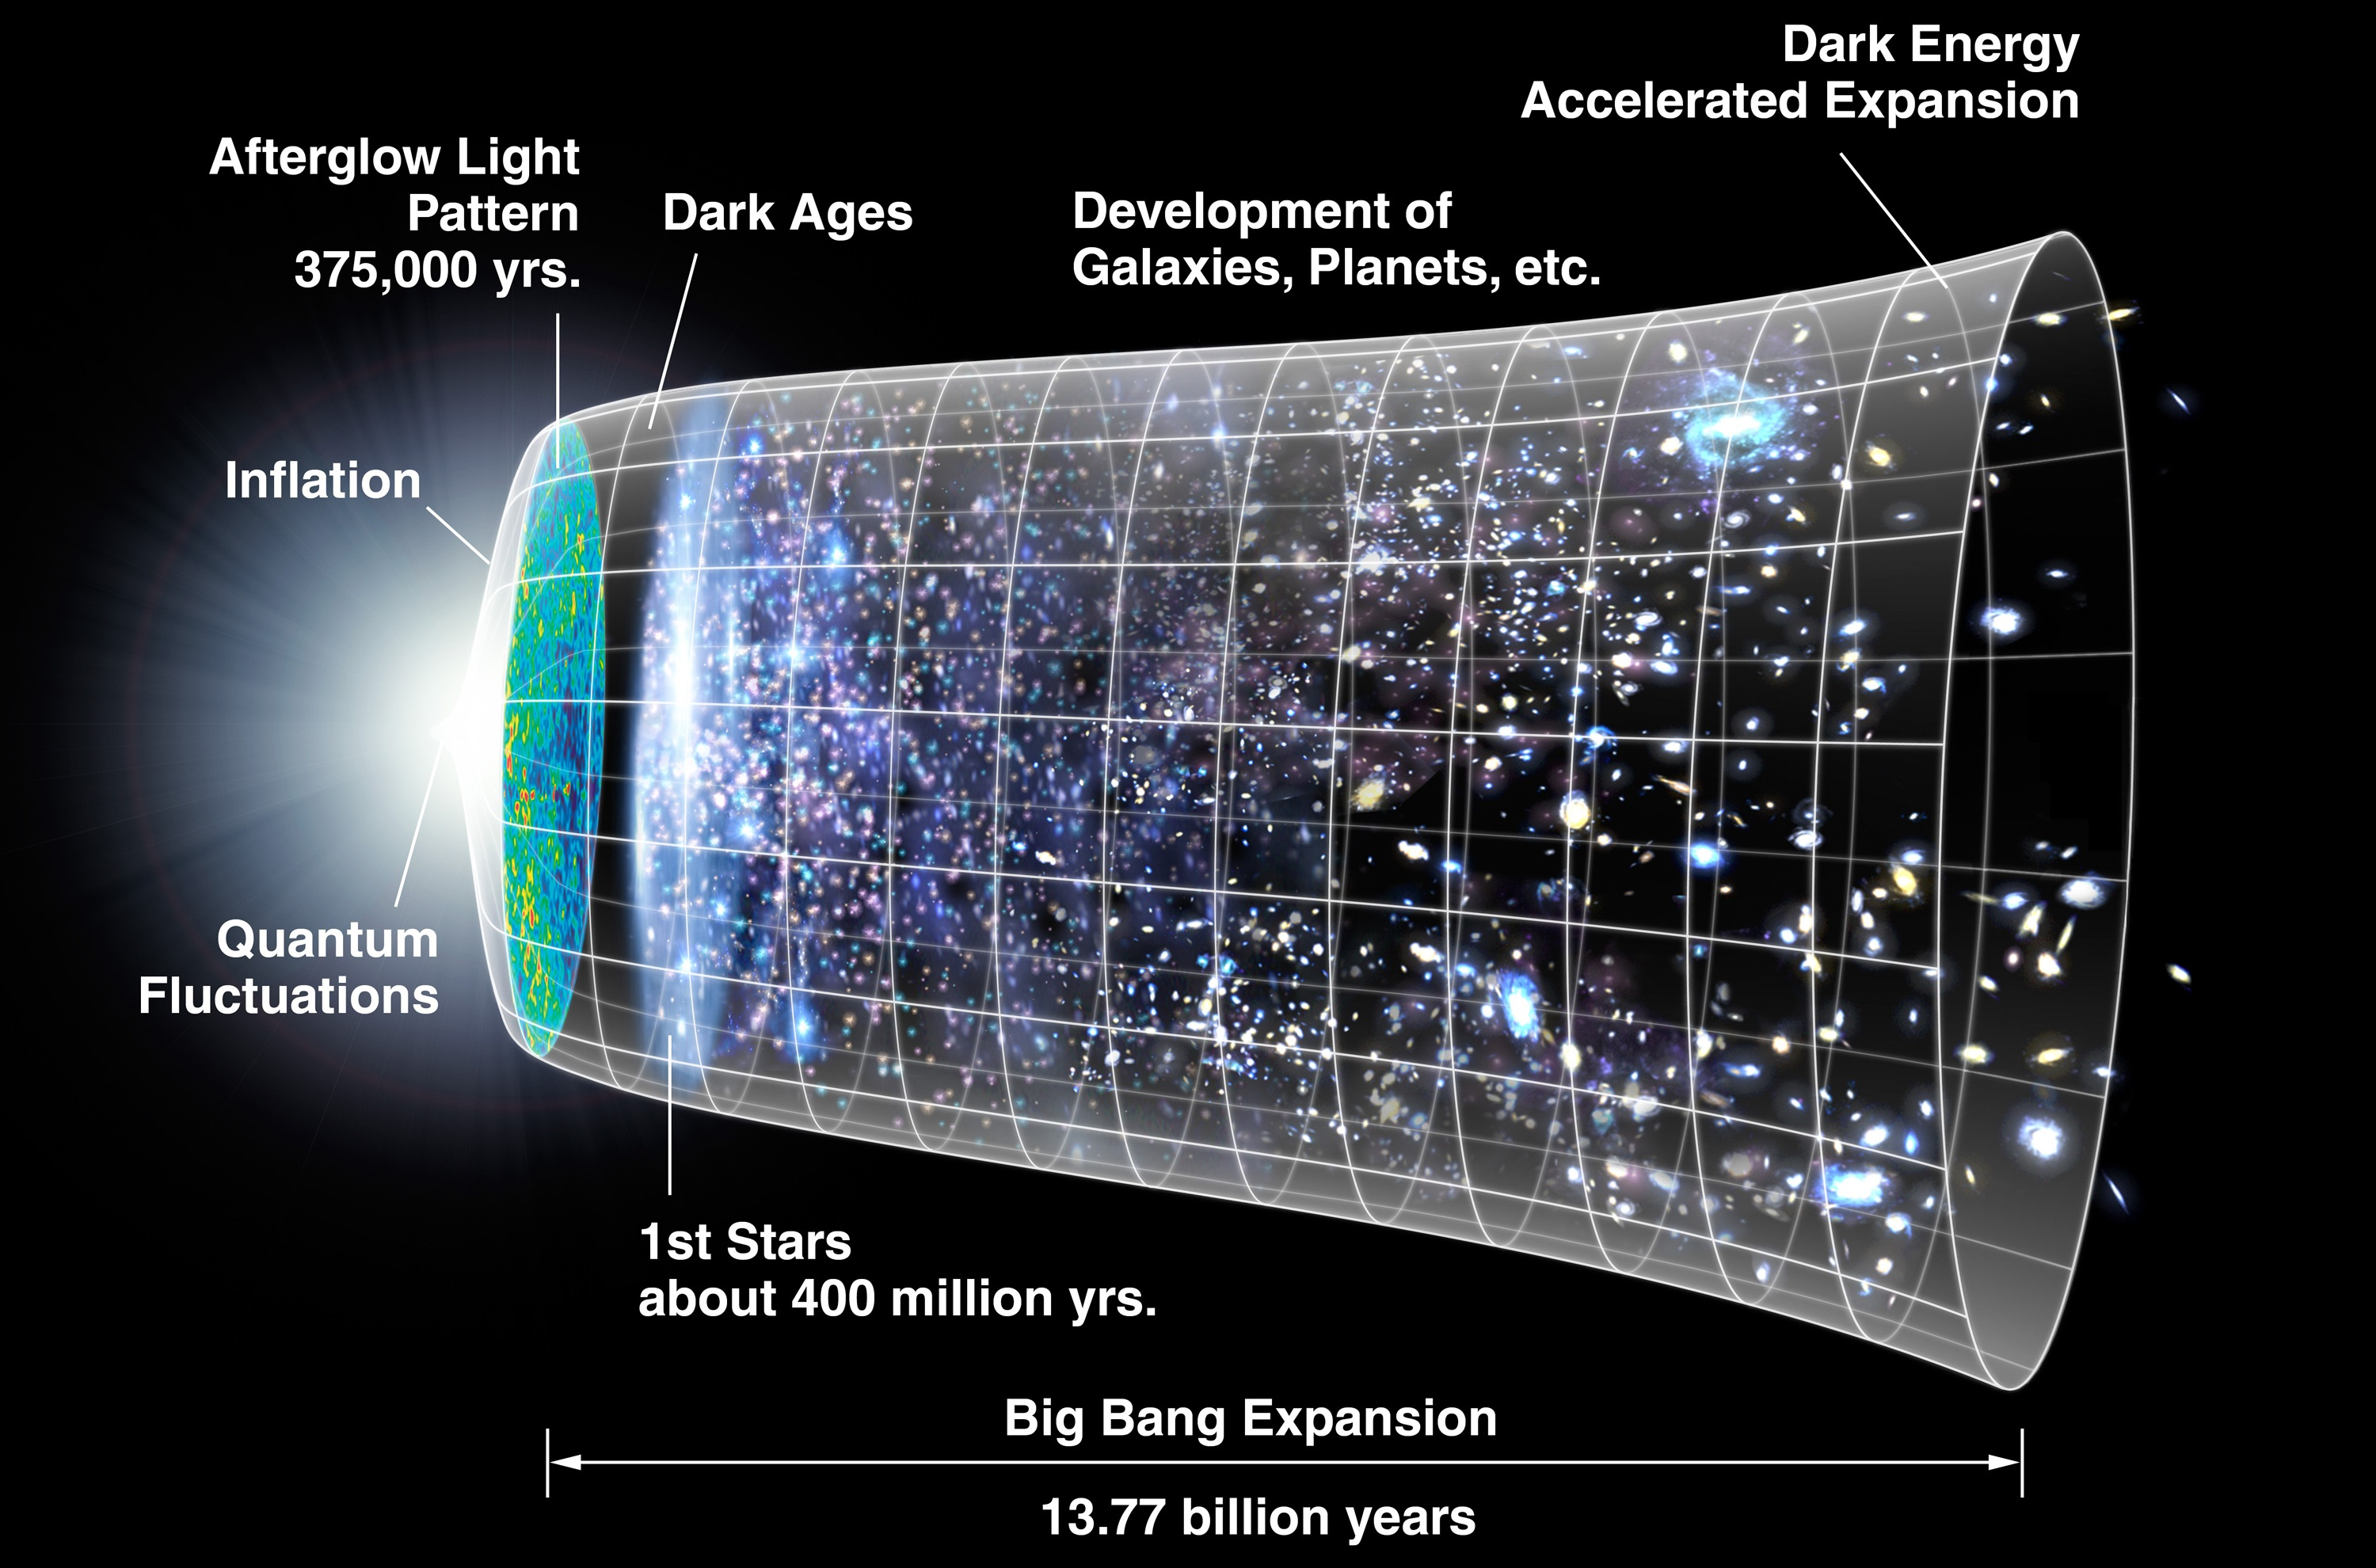
\includegraphics[width=15cm]{bigbang.jpg}
    \caption{\centering \footnotesize{Timeline of the expansion of the universe as per the Big Bang Theory (\textit{Time and Size not to Scale})} \protect\cite{bigbangpic}}
    \label{fig:bigbang}
\end{figure}

Matter, some atoms, formed \cite{hubblebigbang} and dominated over the antimatter \cite{britbigbang}.
Under the assumption that Albert Einstein's general theory of relativity correctly describes the relationship between matter and gravitational forces,
gravity brought matter into greater clumps that are known in the current day as our stars, planets, and galaxies
\cite{hubblebigbang}.

With the rapid expansion, the universe released a flood of radiation, alongside the matter, was also released into the new vast space
\cite{britbigbang,spacebigbang}
in the process known as "reheating", which is "the process whereby the inflation's energy density is converted back
into conventional matter after inflation
\cite{reheating}.
The radiation that was released then travelled through space, and the remnants of the early stages of the universe are known
as the cosmic microwave background (CMB) radiation \cite{britbigbang}, seen in figure \ref{fig:cmb}, 
though sometimes also referred to as the "'afterglow' of the Big Bang"
\cite{spacebigbang}.
These measurments are what allow scientists to predict the age of the universe relative to the currently measured rate of expansion of the universe
\cite{hubblebigbang}

\begin{figure} [H]
    \centering
    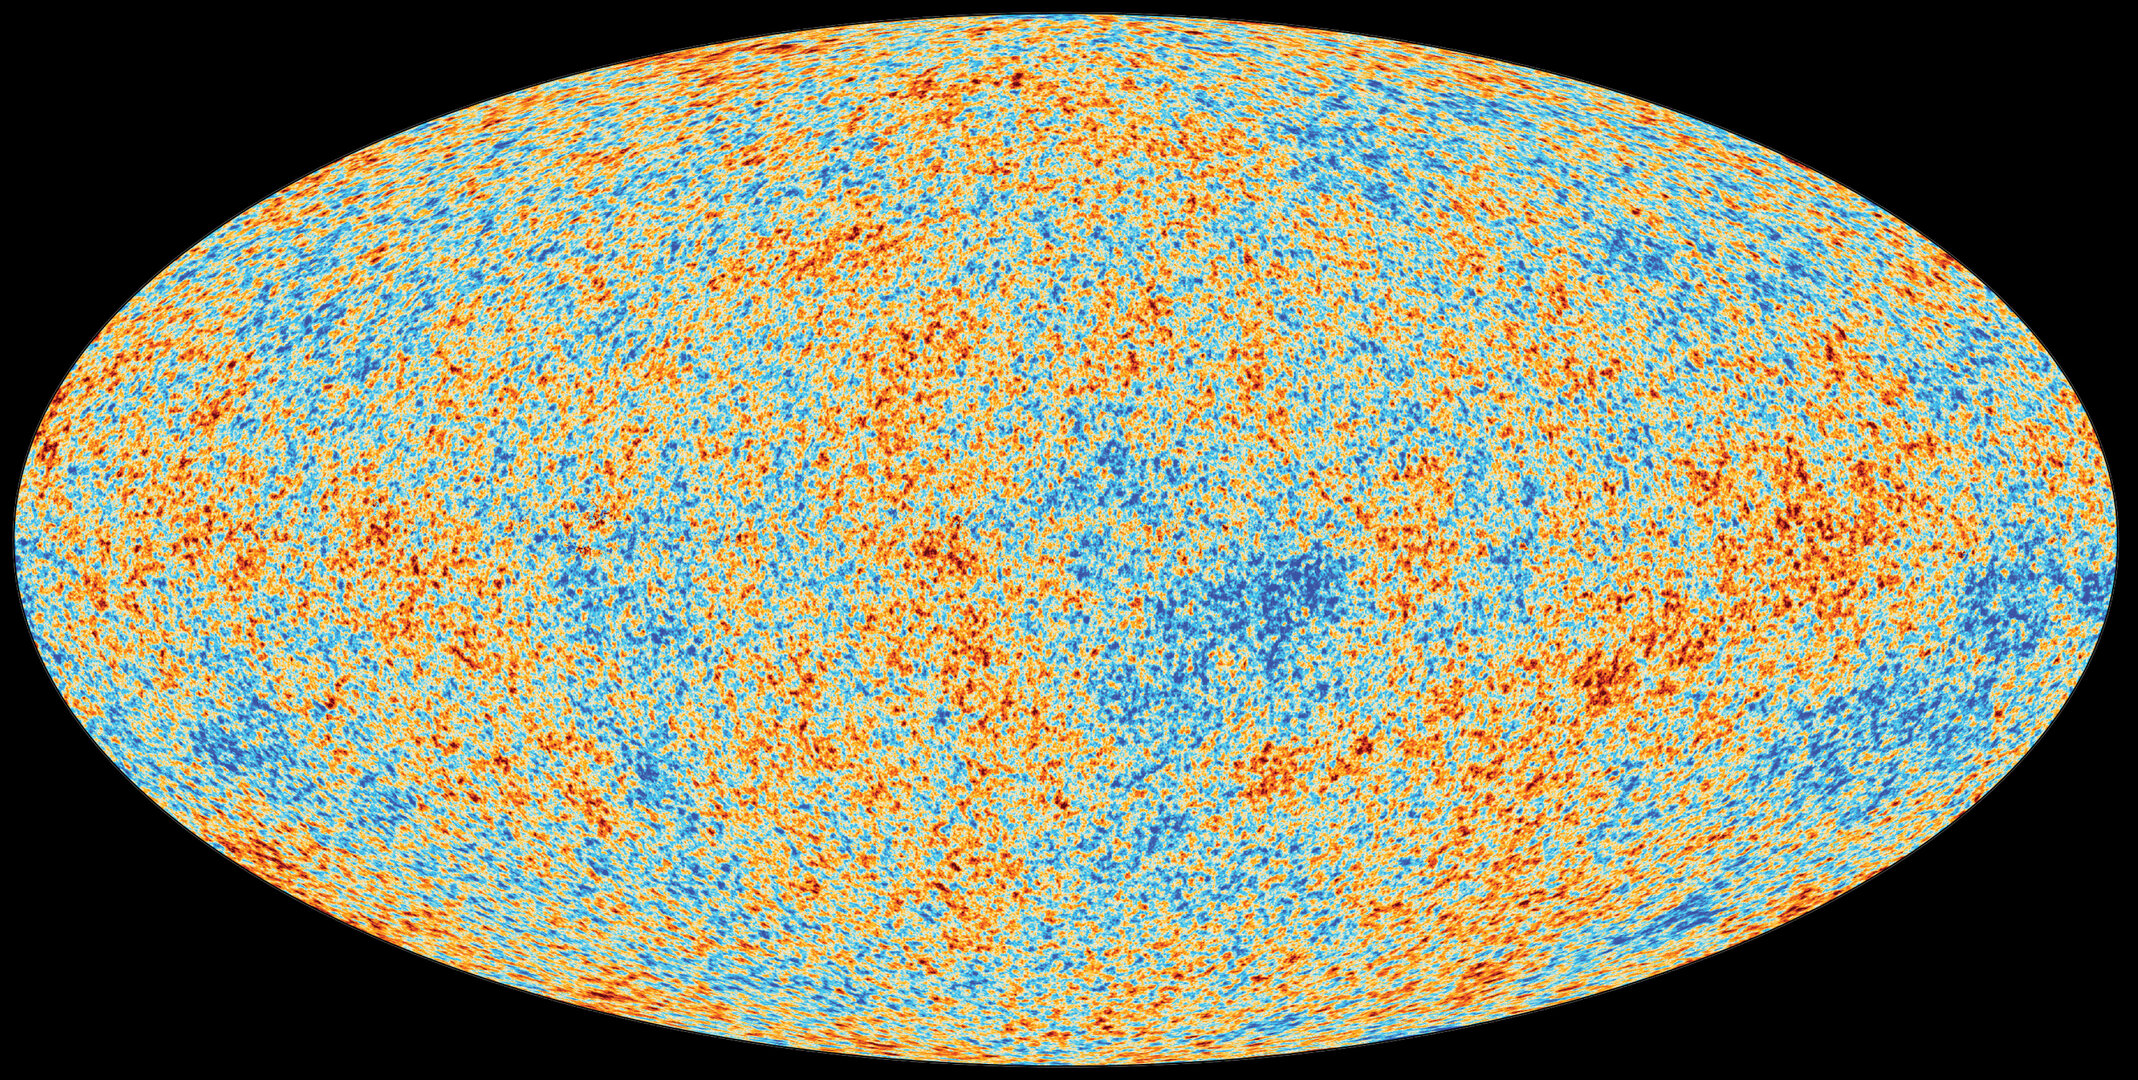
\includegraphics[width=15cm]{cmb.jpg}
    \caption{\centering \footnotesize{Cosmic Microwave Background (CMB) Radiation \protect\cite{cmbpic}}}
    \label{fig:cmb}
\end{figure}

\subsection{Spectrum, Spectrometry, Spectroscopy} \label{sec:1.2}

The electromagnetic spectrum describes all forms of electromagnetic radiation, including visible light, as it varies with wavelength
and frequency  
\cite{britspectra,hubblespectra}.
Spectroscopes are equipments used to visually observe the spectra and spectrographs photograph and map the studied spectra
\cite{britspectra}.
There are three main ways that the spectra can be classified, as illustrated in figure \ref{fig:spectra} \cite{spectrapic}:

\begin{itemize}
    \item \textbf{The continuous spectrum} contains all light emitted in a certain range from hot, dense light sources (like stars)
    from which the radiation travels out in all directions through space. The range of colours emitted depends on the temperature.
    \item \textbf{The absorption spectrum} is measured when light from a continuous source, like a star, passes through a cloud of cooler gas.
    The wavelengths that will be absorbed depend on the composition and elements of the gas, as well as its temperature and density. The wavelengths
    that didn't pass through are what appear as dark lines on the continuous spectrum known as the absorption line spectrum \cite{cosmosabsorp}.
    \item \textbf{The emmission spectrum} is measured when atoms become excited after light, like from a star, passes through a cloud of gas.
    The light can heat up the cloud of gas, thus exciting the atoms and causing them to release light. The light which the gas releases depends on the
    composition and elements, temperature, and density of the gas cloud. The light emitted will appear as coloured lines.
\end{itemize}

\textbf{Spectroscopy} studies the absorption and emission of light and matter radiation \cite{britspectrosco} and how matter would theoretically interact with radiation \cite{ataspectrosco}.
It provides the theoretical backbone to quantum research, particularly on the atomicc structure and radiation
\cite{ataspectrosco}.

\textbf{Spectrometry} puts quantitative values to the theory explored by spectroscopy by measuring the interactions between light (electromagnetic radiation)
and matter
\cite{ataspectrosco}.

\begin{figure}[H]
    \centering
    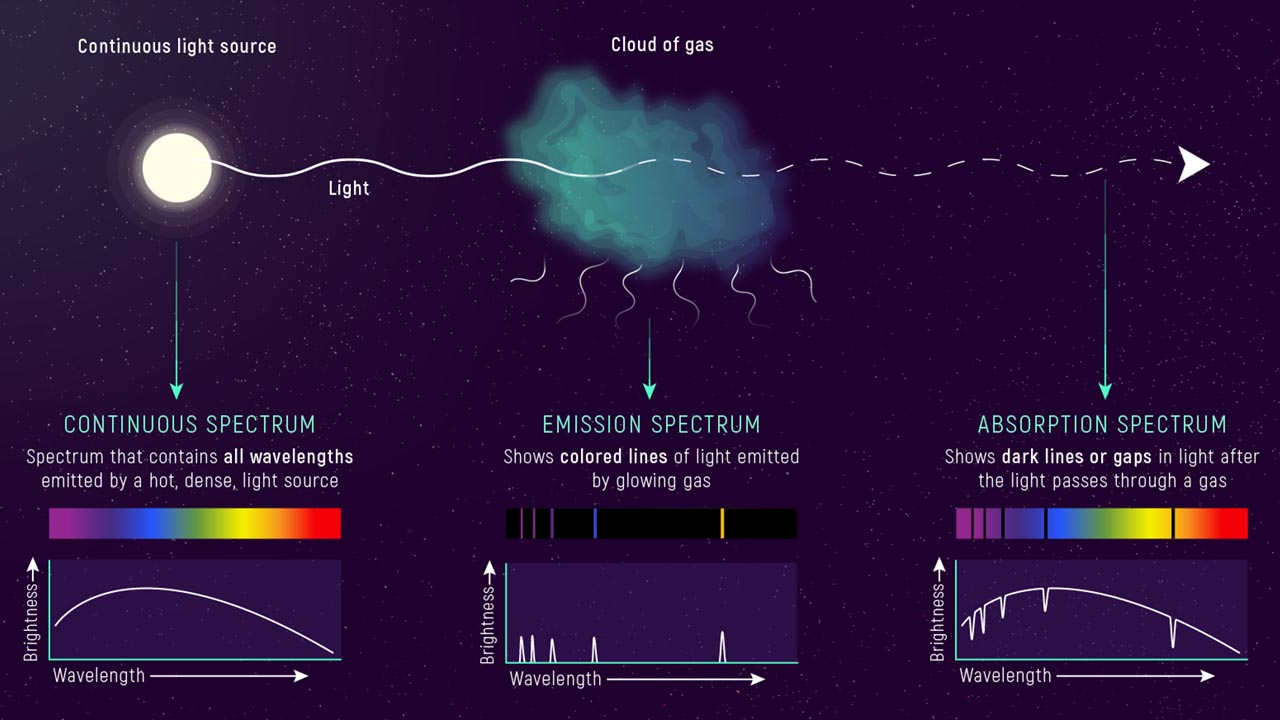
\includegraphics[width=15cm]{spectra.jpg}
    \caption{\centering \footnotesize{Types of spectra: continuous, emission, absorption \protect\cite{spectrapic}}}
    \label{fig:spectra}
\end{figure}

The understanding of electromagnetic spectra is essential in the sudy of the universe. Radio waves and microwaves have the lowest energies and longest wavelengths, as seen in
figure \ref{fig:wavelength}, which allows them to pierce dense stellar dust and gas clouds
\cite{hubblespectra}.
Infrared light can measure the molecular make-up of different stars and planets within our solar system.
The light seen emitted by majority of stars is within our visible light spectrum, which is quite narrow. Hotter stars have more energy and therefore shorter wavelengths
which makes them appear bluer in colour, whereas cooler stars have less energy and so longer wavelengths making them appear redder in colour
\cite{hubblespectra}.
Ultraviolet (UV) can be used to locate and identify the hottest (more energetic) stars as well as stellar nurseries.
X-rays and gamma rays, the most energetic light with the smallest wavelengths, are emitted mostly from materials around a black hole or from
the incredibly energetic and bright, and unstable, neutron stars
\cite{hubblespectra}.

\begin{figure}[H]
    \centering
    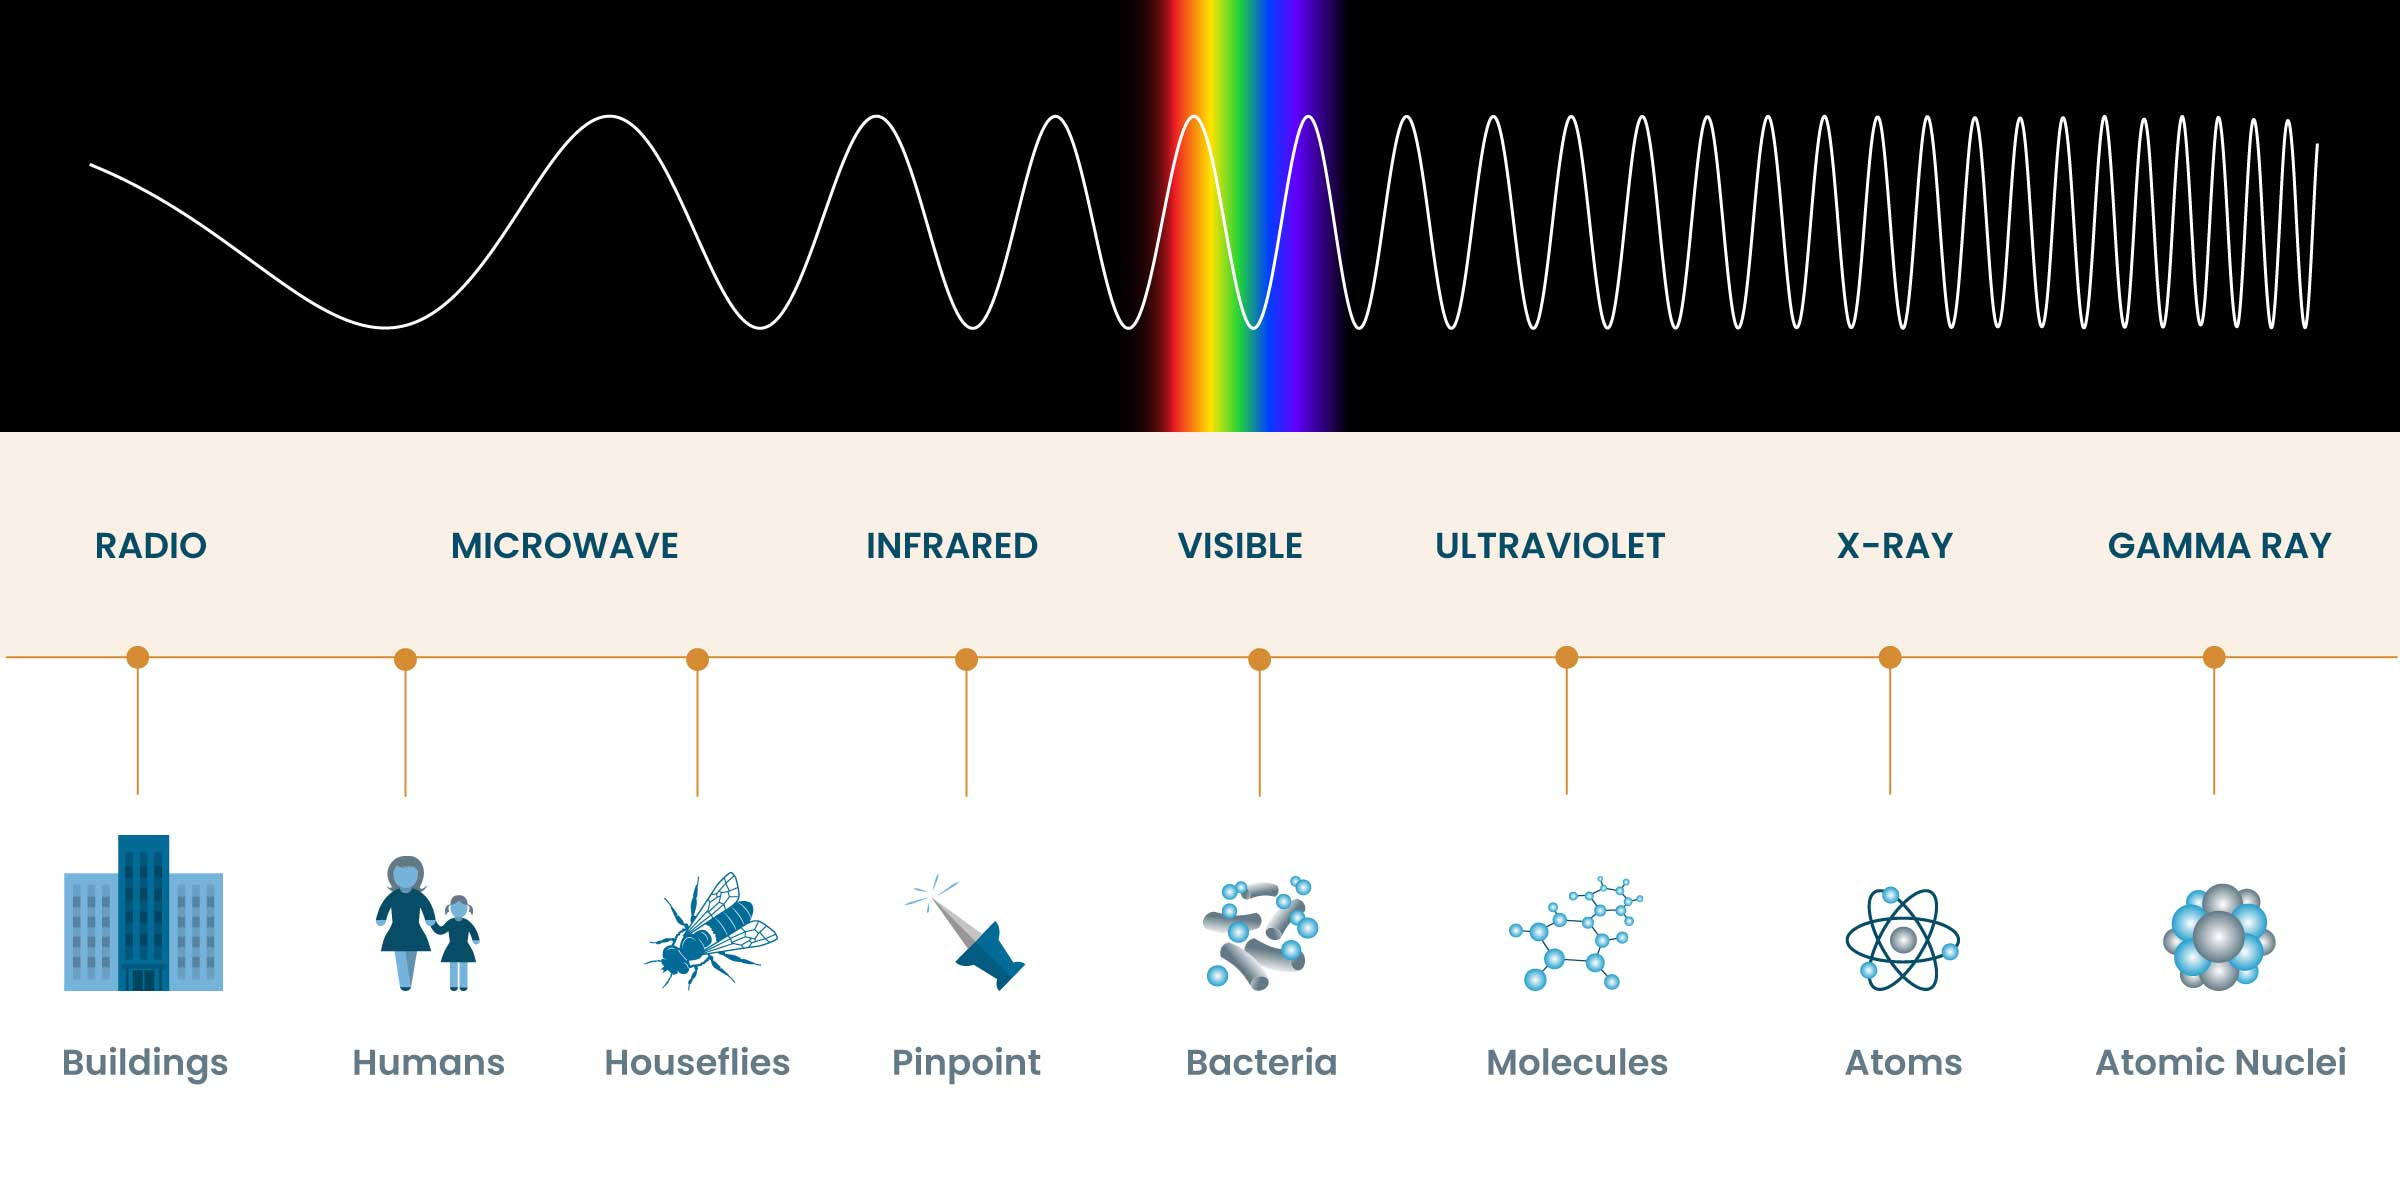
\includegraphics[width=15cm]{light waves.jpg}
    \caption{\centering \footnotesize{Comparison of different types of light, including wavelength size, and frequency \protect\cite{hubblespectra}}}
    \label{fig:wavelength}
\end{figure}

\subsubsection{What is 'Redshift'?} \label{sec:1.2.1}

Redshift is a fundamental concept that explains the continuous expansion of the universe.
It can be interpreted literally as the wavelength of a source being stretched as it moves away, similar to how the wavelength would compress if it were moving towards the viewer (blueshift)
\cite{esaredshift,earthskyredshift}.
As the wavelength stretches, from what was covered in §\ref{sec:1.2}, the colour of the light shifts redder
\cite{esaredshift}.
These are the basic principles of the 'Doppler Effect', which also applies to sound waves
\cite{esaredshift,lcoredshift,britredshift,earthskyredshift}.

It was the scientist Edwin Hubble that reported and named this curiosity after witnessing a distant galaxy receding from the Milky Way system in 1929, hence the 
'Hubble Parameter' covered in §\ref{sec:1.3}
\cite{britredshift}.

This does not mean, however, that the galaxies themselves are moving but rather the fabric of space itself is expanding
\cite{esaredshift}.
In figure \ref{fig:redshift} it is seen how the absorption lines (covered in §\ref{sec:1.2}) shift in colour further up and into the red part
of the electromagnetic spectrum, hence the 'redshift'
\cite{earthskyredshift}.

\begin{figure}[H]
    \centering
    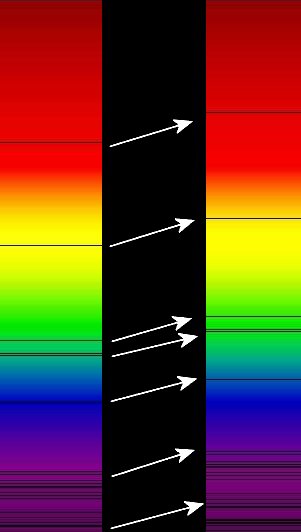
\includegraphics[width=5cm]{Redshift.png}
    \caption{\centering \footnotesize{The dark absorption lines of a star at rest (\textit{left}) get shifted towards red if the star is moving away from Earth (\textit{right}) \protect\cite{earthskyredshift} (via Wikipedia)}}
    \label{fig:redshift}
\end{figure}

Redshift can be observed even in the early stages of the universe's expansion with the CMB radiation seen in figure \ref{fig:cmb}, §\ref{sec:1.1.1}.

\subsection{The Hubble Parameter} \label{sec:1.3}



\subsection{H and K Lines} \label{sec:1.4}

\subsection{More Terminology} \label{sec:1.5}

\section{The Procedure} 



\section{Results and Calculations}



\section{Conclusion}



\section{Applications of the Hubble Constant}




\newpage


%%%%%%%%%%%%%%%%%%%%%%%%%%%%%%%%%%%

\bibliographystyle{IEEEtran}
\bibliography{References}

\newpage

\section*{Appendix}
\addcontentsline{toc}{section}{Appendix}

\subsection*{Raw Data}
\addcontentsline{toc}{subsection}{Raw Data}

\listoffigures


\end{document}